% Provenance (never printed): see sources/outline_sources.md (Year 3:
% stereographic projection; fold and fault analysis; palaeostress; balanced
% cross-sections). Brief: sources/book5/BRIEFS.md, ch. 8. Nets, pi-diagram and
% fault-slip data from figdata/bachelor-3/stereonet.py (Varden data invented,
% from figdata/shared/region.py); Fry plot from figdata/bachelor-3/fry.py.
% Exercise and problem values in the Book 5 scratch calculator calc/ch08.py.
% No real-world numbers: no ledger rows.
\chapter{Structurele analyse}\label{ch:b3:structural-analysis}

Een geoloog heeft tweehonderd gelaagdheidsvlakken gemeten op de flanken van een plooi
die te groot is om in één keer te overzien: het scharnier ligt onder een bos, de flanken lopen kilometers ver
door. Elke meting is een paar getallen. Uitgezet als punten in een cirkelvormig diagram
vallen de polen van de vlakken langs één kromme, een grootcirkel, en
de \omterm{def:b3:structural-analysis:stereo}{pool} van die grootcirkel is de plooias, een lijn die niemand ooit heeft gezien.
Dit hoofdstuk bouwt het diagram, de \omterm{def:b3:structural-analysis:stereo}{stereografische projectie} en gebruikt die
samen met de vectorgereedschappen erachter om plooiassen te vinden, de rek te meten
die vervormde objecten hebben vastgelegd, de spanning te herstellen die een reeks
breuken heeft aangedreven, en een vervormde doorsnede terug te brengen naar de toestand van vóór de
vervorming.

\begin{recall}
Grootcirkels en kleine cirkels van een bol staan in Boek~3, in het hoofdstuk
over sferische astronomie; strekking, helling, hellingrichting, richting en duik in de
hoofdstukken over geologische kaarten en doorsneden; de naar boven gerichte eenheidsnormaal van een
vlak met hellingrichting $\alpha$ en helling $\delta$, $\vec n = (\sin\delta
\sin\alpha, \sin\delta\cos\alpha, \cos\delta)$ in oost-, noord- en opwaartse
componenten, en het vectorgemiddelde van een reeks metingen in het eerste hoofdstuk over
veld- en laboratoriummethoden. Plooielementen en -klassen, de scharnierlijn van een
plooi evenwijdig aan $\vec n_1\times\vec n_2$ en de interflankhoek
$\ang{180} - \arccos(\vec n_1\cdot\vec n_2)$, evenals Andersons theorie van
breukvorming, staan in het hoofdstuk over breuken, plooien en fabrieken; spanning, de
hoofdspanningen, de rekellips en de eenvoudige schuif in het hoofdstuk over
spanning, rek en reologie; de rake van een glijvector (uit de strekking,
\ang{-90} voor een afschuiving, \ang{90} voor een opschuiving, 0 sinistraal en
\ang{180} dextraal) en de P- en T-assen van een haardmechanisme in het hoofdstuk over
de aardbevingsbron. De uitgebalanceerde doorsnede en het décollement staan in
Boek~4, in het hoofdstuk over de Alpen. De kleinste kwadraten staan in
\cref{sec:b3:seismology-imaging:inverse}; eigenwaarden en eigenvectoren van een
symmetrische matrix staan in de wiskundeboeken.
\end{recall}

\section{De stereografische projectie}\label{sec:b3:structural-analysis:stereo}

De gegevens van een geoloog zijn oriëntaties: de stand van een gelaagdheidsvlak, een
breuk, een foliatie; de richting en duik van een lineatie, een plooischarnier, een glijrichting.
Elk ervan is een richting door een punt, zonder positie. Om er honderden met elkaar te vergelijken,
denke men ze zich allemaal verplaatst naar het middelpunt van één bol:
een lijn snijdt de onderhelft van de bol in één punt, een vlak snijdt haar langs
een halve grootcirkel. Een diagram van de onderhelft toont dan lijnen als
punten en vlakken als krommen.

\begin{definition}[Stereografische projectie, hoekgetrouw net, oppervlaktegetrouwe projectie, pool]\label{def:b3:structural-analysis:stereo}
Laat een lijn door het middelpunt $O$ van een bol met straal $R$ de onderhelft
snijden in $P$, onder de hoek $\theta = \ang{90} - p$ vanaf het nadir, waarin
$p$ de duik van de lijn is en $t$ haar richting. De \emph{stereografische
projectie}\index{stereografische projectie} brengt $P$ over op het punt waar de rechte lijn van het zenit naar $P$
snijdt de horizontale vlakte door $O$; dat punt ligt op de afstand $r$ van $O$ in
het azimuth $t$. Het diagram van de onderhelft, zo getekend, met zijn rooster van
grootcirkels en kleine cirkels,
is het \emph{hoekgetrouw net}\index{hoekgetrouw net} (of
Wulffnet). De \emph{oppervlaktegetrouwe projectie (van de bol)}\index{oppervlaktegetrouwe projectie (van de bol)}
brengt $P$ over op het punt op de afstand $r =
R\sqrt2\sin(\theta/2)$ in het azimuth $t$; haar net is het Schmidtnet. De
\emph{pool}\index{pool (van een vlak)} van een vlak is zijn normaallijn, uitgezet als
een punt: voor een vlak met hellingrichting $\alpha$ en helling $\delta$, de pool
heeft een richting $\alpha + \ang{180}$ en een duik $\ang{90} - \delta$.
\end{definition}

Beide projecties leggen een verticale lijn in het midden en een horizontale lijn op
de cirkel met straal $R$, de primitieve. Ze verschillen in wat ze bewaren.

\begin{theorem}[De twee projecties]\label{thm:b3:structural-analysis:projections}
\begin{enumerate}[label=(\alph*)]
  \item De \omterm{def:b3:structural-analysis:stereo}{stereografische projectie} plaatst $P$ op $r = R\tan(\theta/2)$. Ze is
        conform: op elk punt rekt ze alle richtingen met dezelfde
        factor, $1/(2\cos^2(\theta/2))$, zodat ze de hoeken tussen
        krommen bewaart.
  \item De oppervlaktegetrouwe projectie vermenigvuldigt elk oppervlak met dezelfde factor,
        $1/2$: het oppervlak van een gebied op het net is de helft van het oppervlak
        van het gebied op de halve bol dat het voorstelt.
\end{enumerate}
\end{theorem}

\begin{proof}
(a) In het verticale vlak door het zenit $Z$, het nadir en $P$
(eerste figuur hieronder), spant de boog van het nadir tot $P$
de hoek $\theta$ op in het middelpunt, dus de ingeschreven hoek
$\theta/2$ in $Z$, dat op de afstand $R$ boven $O$ ligt: $r =
R\tan(\theta/2)$. Een kleine stap $R\,\mathrm d\theta$ op de bol richting het
nadir wordt $\mathrm dr = R\,\mathrm d\theta/(2\cos^2(\theta/2))$ op het
diagram. De cirkel van punten op de hoek $\theta$ van het nadir heeft de
omtrek $2\pi R\sin\theta$ en wordt een cirkel met omtrek $2\pi
r$; de verhouding is $\tan(\theta/2)/\sin\theta = 1/(2\cos^2(\theta/2))$, dezelfde
als langs de straal. Een afbeelding die in twee loodrechte
richtingen even sterk rekt, rekt in alle richtingen even sterk en bewaart hoeken.

(b) De kalot van de bol binnen de hoek $\theta$ van het nadir heeft het oppervlak
$2\pi R^2(1 - \cos\theta) = 4\pi R^2\sin^2(\theta/2)$; haar beeld is de schijf
met oppervlak $\pi r^2 = 2\pi R^2\sin^2(\theta/2)$, de helft ervan. Beide oppervlakken worden
gelijkmatig verdeeld over het azimuth, dus de sector van de kalot tussen twee azimuts
en haar beeld houden de verhouding $1/2$, en dat geldt ook voor de ring tussen twee waarden
van $\theta$, het verschil van twee kalotten. Elk gebied is een vereniging van zulke
kleine ringsectoren.
\end{proof}

De \omterm{def:b3:structural-analysis:stereo}{stereografische projectie} brengt ook elke cirkel van de bol, groot of
klein, over op een cirkel of een rechte lijn op het diagram; dat nemen we aan. Ze maakt het
hoekgetrouwe net eenvoudig met passer te tekenen, en een kleine cirkel, de kegel van
de lijnen op een vaste hoek van een as, behoudt haar vorm. De oppervlaktegetrouwe
projectie vervormt vormen: een kleine cirkel wordt een ovaal, uitgerekt
langs de primitieve. Het is de projectie waarop een wolk van polen geteld kan worden,
omdat een gelijk oppervlak van het net een gelijk deel van de
richtingen van de halve bol bevat; structurele geologen, en seismologen voor hun
haardmechanismen, gebruiken haar voor hun gegevens.

\begin{omfigure}
\begin{tikzpicture}[scale=1.0, >=stealth]
% (a) equal-angle: theta = 60 deg, R = 2 cm; r = 2 tan 30 = 1.155
\begin{scope}
\draw[thick] (0,0) circle (2);
\draw (-2.5,0) -- (2.5,0) node[right, font=\scriptsize] {vlak};
\fill (0,2) circle (1.5pt) node[above, font=\scriptsize] {zenit $Z$};
\fill (0,-2) circle (1.5pt) node[below, font=\scriptsize] {nadir};
\fill (0,0) circle (1.2pt) node[above left, font=\scriptsize] {$O$};
\draw[dashed] (0,2) -- (0,-2);
\draw[omDef, thick] (0,0) -- (1.732,-1);
\fill[omDef] (1.732,-1) circle (1.5pt) node[below right, font=\scriptsize] {$P$};
\draw[omThm] (0,2) -- (1.732,-1);
\fill[omThm] (1.155,0) circle (1.5pt);
\node[omThm, font=\scriptsize, above right] at (1.155,0) {$P'$};
\draw (0,-0.6) arc[start angle=-90, end angle=-30, radius=0.6];
\node[font=\scriptsize] at (0.38,-0.85) {$\theta$};
\draw (0,1.2) arc[start angle=-90, end angle=-60, radius=0.8];
\node[font=\scriptsize] at (0.25,0.95) {$\theta/2$};
\draw[<->] (0,0.25) -- (1.155,0.25);
\node[font=\scriptsize, above] at (0.58,0.25) {$r$};
\node[font=\small] at (0,-3.0) {(a) hoekgetrouw};
\end{scope}
% (b) equal-area: chord from nadir to P = 2R sin(theta/2) = 2
\begin{scope}[xshift=6.6cm]
\draw[thick] (0,0) circle (2);
\draw (-2.5,0) -- (2.5,0);
\draw (-2.5,-2) -- (2.5,-2) node[right, font=\scriptsize] {raakvlak};
\fill (0,-2) circle (1.5pt) node[below left, font=\scriptsize] {nadir};
\fill (0,0) circle (1.2pt) node[above left, font=\scriptsize] {$O$};
\draw[dashed] (0,2) -- (0,-2);
\draw[omDef, thick] (0,0) -- (1.732,-1);
\fill[omDef] (1.732,-1) circle (1.5pt) node[above right, font=\scriptsize] {$P$};
\draw[omThm] (0,-2) -- (1.732,-1);
\draw[omThm, dashed] (1.732,-1) arc[start angle=30, end angle=0, radius=2];
\fill[omThm] (2,-2) circle (1.5pt);
\node[omThm, font=\scriptsize, below] at (2,-2.05) {$2R\sin(\theta/2)$};
\draw (0,-0.6) arc[start angle=-90, end angle=-30, radius=0.6];
\node[font=\scriptsize] at (0.38,-0.85) {$\theta$};
\node[font=\small] at (0,-3.0) {(b) oppervlaktegetrouw};
\end{scope}
\end{tikzpicture}

\par\smallskip{\small De twee projecties, in het verticale vlak door de
lijn $OP$. (a) De \omterm{def:b3:structural-analysis:stereo}{stereografische projectie} brengt $P$ over naar $P'$, waar de lijn
vanuit het zenit het horizontale vlak snijdt: de hoek bij $Z$ is
$\theta/2$, dus $r = R\tan(\theta/2)$. (b) De oppervlaktegetrouwe projectie brengt
$P$, rond het nadir, over op het raakvlak op de afstand $2R\sin(\theta/2)$
van de koorde; het beeld wordt daarna geschaald met $1/\sqrt2$ zodat de horizontale
lijnen op een primitieve met straal $R$ vallen.}\label{fig:b3:structural-analysis:geometry}
\end{omfigure}

\begin{omfigure}
\begin{tikzpicture}
\begin{groupplot}[group style={group size=2 by 1, horizontal sep=0.8cm},
  width=0.5\linewidth, height=0.5\linewidth, axis equal image, hide axis,
  xmin=-1.15, xmax=1.15, ymin=-1.15, ymax=1.15, unbounded coords=jump,
  title style={font=\small}]
\nextgroupplot[title={(a) hoekgetrouw (Wulff) net}]
% computed in figdata/bachelor-3/stereonet.py
\addplot[gray!75, very thin] table[x=x, y=y] {figdata/out/bachelor-3-stereonet-wulff.dat};
\addplot[gray!75, very thin] coordinates {(-1,0) (1,0)};
\addplot[black, thick, domain=0:360, samples=181] ({cos(x)}, {sin(x)});
\node[font=\scriptsize, above] at (axis cs:0,1.0) {N};
\nextgroupplot[title={(b) oppervlaktegetrouw (Schmidt) net}]
\addplot[gray!75, very thin] table[x=x, y=y] {figdata/out/bachelor-3-stereonet-schmidt.dat};
\addplot[gray!75, very thin] coordinates {(-1,0) (1,0)};
\addplot[black, thick, domain=0:360, samples=181] ({cos(x)}, {sin(x)});
\node[font=\scriptsize, above] at (axis cs:0,1.0) {N};
\end{groupplot}
\end{tikzpicture}

\par\smallskip{\small De twee netten, getekend uit de formules van de stelling
hierboven: grootcirkels van de vlakken met strekking noord--zuid en helling die elke
\ang{10} naar oost en west verandert, en kleine cirkels elke \ang{10} rond de
noord--zuidas. Op het hoekgetrouwe net zijn de kleine cirkels cirkels; op het
oppervlaktegetrouwe net zijn ze ovalen, maar gelijke oppervlakken bevatten gelijke delen van de
richtingen.}\label{fig:b3:structural-analysis:nets}
\end{omfigure}

\paragraph{Vlakken, lijnen en hoeken.}
Een vlak met hellingrichting $\alpha$ en helling $\delta$ snijdt de onderste halve bol
langs een halve grootcirkel. De uiteinden liggen op de primitieve aan de twee uiteinden van
de strekking; het midden is de lijn van steilste helling, die onder $\delta$ duikt
richting $\alpha$; en zijn \omterm{def:b3:structural-analysis:stereo}{pool} ligt \ang{90} van elk punt ervan, in het
azimut $\alpha + \ang{180}$. Een lijn in het vlak is een punt op de grootcirkel.
Om gegevens uit te zetten wordt een doorzichtige overlay op het net gelegd en
om het middelpunt gedraaid tot de strekking van de gegevens langs de noord--zuiddiameter van het net ligt;
daarna wordt de grootcirkel van de juiste helling getekend, en wordt de overlay weer teruggedraaid.
De hoek tussen twee lijnen wordt gemeten langs de grootcirkel door beide punten,
door de verdelingen van de kleine cirkels te tellen die hij kruist, nadat de overlay
is gedraaid tot beide punten op één grootcirkel van het net liggen. De hoek tussen
twee vlakken is de hoek tussen hun polen, of het supplement daarvan.
Een computer doet hetzelfde met vectoren: de hoek tussen twee lijnen van eenheidsvectoren
$\vec u$ en $\vec v$ is $\arccos|\vec u\cdot\vec v|$.

\begin{method}[Rotatie van gegevens om een as]\label{met:b3:structural-analysis:rotation}
Om een kanteling ongedaan te maken, bijvoorbeeld om een laag weer horizontaal te brengen met de
lineaties die erin zitten, of om een paleomagnetische richting te herstellen die is gemeten in
gekantelde lagen (in \cref{ch:b3:palaeomagnetism}):
\begin{enumerate}
  \item Kies de rotatieas: voor een gekantelde laag de strekkingslijn ervan, horizontaal;
        de hoek is de helling, in de zin die de laag omhoog brengt.
  \item Draai op het net de overlay tot de as langs de
        noord--zuiddiameter ligt, waar de kleine cirkels de kegels rond de
        as vormen.
  \item Verplaats elk punt langs zijn kleine cirkel over de rotatiehoek,
        gemeten op de grootcirkels. Een punt dat de onderste halve bol zou verlaten,
        verschijnt weer aan het andere eind van zijn kleine cirkel, in het
        tegengestelde azimut.
  \item Draai de overlay terug. Met vectoren is de rotatie van $\vec v$ over de
        hoek $\omega$ om de eenheidsas $\vec k$ is $\vec v' = \vec v
        \cos\omega + (\vec k\times\vec v)\sin\omega + \vec k(\vec k\cdot\vec
        v)(1 - \cos\omega)$.
\end{enumerate}
\end{method}

\section{Plooianalyse}\label{sec:b3:structural-analysis:folds}

Een cilindrische plooi ontstaat doordat een rechte lijn, de plooias,
evenwijdig aan zichzelf wordt verplaatst. Elk vlak dat het geplooide oppervlak raakt, bevat de as,
dus staat elke normaal op het oppervlak loodrecht op de as:
alle polen liggen op de grootcirkel van het vlak loodrecht op de as.

\begin{definition}[Pi-diagram, bèta-as]\label{def:b3:structural-analysis:pi}
Het \emph{pi-diagram}\index{pi-diagram} van een plooi is de weergave van de polen van
de vlakken die op het geplooide oppervlak zijn gemeten. Bij een cilindrische plooi liggen ze op
een grootcirkel, de $\pi$-gordel; de \omterm{def:b3:structural-analysis:stereo}{pool} van de gordel is de
\emph{bèta-as}\index{bèta-as}, de schatting van de plooias op basis van de
metingen.
\end{definition}

Bij slechts twee flanken is de \omterm{def:b3:structural-analysis:pi}{bèta-as} het uitproduct van hun normalen,
zoals Boek~3 voor de scharnierlijn liet zien. Bij tweehonderd verspreide
metingen is een best fit nodig. Het vectorgemiddelde, dat voor de metingen
van één vlak diende, voldoet niet: de polen van een gordel wijzen langs die gordel in alle richtingen, en
hun gemiddelde zegt weinig over de cirkel waarop zij liggen.

\begin{definition}[Oriëntatietensor]\label{def:b3:structural-analysis:orientation-tensor}
De \emph{oriëntatietensor}\index{oriëntatietensor} van $N$ eenheidsvectoren
$\vec p_1, \dots, \vec p_N$ is de symmetrische matrix
\[
  T = \frac1N\sum_{i=1}^N \vec p_i\,\vec p_i^{\mathsf T},
  \qquad T_{jk} = \frac1N\sum_i p_{ij}\,p_{ik} .
\]
Zij verandert niet wanneer een vector door zijn tegengestelde wordt vervangen, en is daarom geschikt voor
assen en polen, die geen richting hebben. Haar eigenwaarden $\lambda_1 \ge \lambda_2
\ge \lambda_3 \ge 0$ tellen op tot het spoor, $1$.
\end{definition}

\begin{theorem}[Cluster en gordel uit de oriëntatietensor]\label{thm:b3:structural-analysis:tensor}
Voor elke eenheidsvector $\vec u$ geldt
\[
  \frac1N\sum_{i=1}^N (\vec p_i\cdot\vec u)^2 = \vec u^{\mathsf T}T\,\vec u ,
\]
Dit neemt zijn kleinste waarde aan, $\lambda_3$, wanneer $\vec u$ de eigenvector
$\vec e_3$ van de kleinste eigenwaarde is, en zijn grootste, $\lambda_1$, langs de
eigenvector $\vec e_1$. Omdat $\vec p_i\cdot\vec u$ de sinus is van de hoek
tussen $\vec p_i$ en het vlak loodrecht op $\vec u$, is de grootcirkel
loodrecht op $\vec e_3$ de gordel die de som van de gekwadrateerde
sinussen van de afstanden van de polen tot die gordel minimaliseert, en $\sqrt{\lambda_3}$ is hun
kwadratisch gemiddelde sinus. De as $\vec e_1$ is de lijn die het dichtst bij de vectoren ligt,
de gemiddelde as van een cluster.
\end{theorem}

\begin{proof}
$(\vec p_i\cdot\vec u)^2 = \vec u^{\mathsf T}\vec p_i\,\vec p_i^{\mathsf T}\vec
u$; neem het gemiddelde over $i$. De matrix $T$ is symmetrisch. Dus heeft zij een orthonormale
basis van eigenvectoren, waarin $\vec u = \sum_k u_k\vec e_k$ met $\sum_k
u_k^2 = 1$ en $\vec u^{\mathsf T}T\vec u = \sum_k\lambda_k u_k^2$. Dit is een
gewogen gemiddelde van de eigenwaarden, met gewichten $u_k^2$ die optellen tot 1: het
ligt tussen $\lambda_3$ en $\lambda_1$ en bereikt ze voor $\vec u = \vec
e_3$ en $\vec e_1$.
\end{proof}

De eigenwaarden beschrijven de vorm van de data. Een cluster heeft $\lambda_1$ dicht bij
1 en de andere twee klein; een gordel heeft $\lambda_3$ dicht bij 0, de polen zijn
over de cirkel gespreid, zodat $\lambda_1$ en $\lambda_2$ de rest delen;
gelijkmatig verspreide vectoren geven drie eigenwaarden dicht bij $1/3$. Een plooi is
cilindrisch binnen de nauwkeurigheid van de metingen, wanneer $\sqrt{\lambda_3}$
niet groter is dan de spreiding van herhaalde metingen van één vlak. Een kegelvormige plooi,
of twee generaties plooien, spreidt de polen weg van elke grootcirkel
en verhoogt $\lambda_3$.

De onderstaande figuur zet twaalf metingen uit van de twee flanken van de Varden-antiklinaal,
de verzonnen plooi van deze reeks (\cref{pb:b3:structural-analysis:1}
berekent de as ervan). De polen van de flauwe flanken clusteren dicht bij het middelpunt van het net
in twee groepen, die samen een gordel vormen die bijna oost--west loopt;
de \omterm{def:b3:structural-analysis:pi}{bèta-as} ligt op de primitieve, bijna precies noord. De gemiddelde
vlakken van de twee flanken, getekend als grootcirkels, snijden elkaar in hetzelfde punt:
de \omterm{def:b3:structural-analysis:pi}{bèta-as} is de lijn die gemeen is aan alle flanken.

\begin{omfigure}
\begin{tikzpicture}
\begin{groupplot}[group style={group size=2 by 1, horizontal sep=1.0cm},
  width=0.5\linewidth, height=0.5\linewidth, axis equal image,
  unbounded coords=jump, title style={font=\small}]
\nextgroupplot[hide axis, xmin=-1.15, xmax=1.15, ymin=-1.15, ymax=1.15,
  title={(a) de onderste halve bol}]
% computed in figdata/bachelor-3/stereonet.py (Varden readings invented)
\addplot[gray!35, very thin] table[x=x, y=y] {figdata/out/bachelor-3-stereonet-schmidt.dat};
\addplot[black, thick, domain=0:360, samples=181] ({cos(x)}, {sin(x)});
\addplot[gray, densely dashed] table[x=x, y=y] {figdata/out/bachelor-3-stereonet-limbs.dat};
\addplot[omDef, thick] table[x=x, y=y] {figdata/out/bachelor-3-stereonet-girdle.dat};
\addplot[only marks, mark=*, mark size=1.2pt] table[x=x, y=y] {figdata/out/bachelor-3-stereonet-poles.dat};
\addplot[only marks, mark=triangle*, mark size=3pt, omThm] table[x=x, y=y] {figdata/out/bachelor-3-stereonet-beta.dat};
\node[font=\scriptsize, above] at (axis cs:0,1.02) {N};
\node[omThm, font=\scriptsize, right] at (axis cs:0.06,0.88) {$\beta$};
\draw[gray] (axis cs:-0.3,-0.3) rectangle (axis cs:0.3,0.3);
\nextgroupplot[xmin=-0.3, xmax=0.3, ymin=-0.3, ymax=0.3, title={(b) het centrum, vergroot},
  xtick=\empty, ytick=\empty]
\addplot[gray!35, very thin] table[x=x, y=y] {figdata/out/bachelor-3-stereonet-schmidt.dat};
\addplot[omDef, thick] table[x=x, y=y] {figdata/out/bachelor-3-stereonet-girdle.dat};
\addplot[only marks, mark=*, mark size=1.5pt] table[x=x, y=y] {figdata/out/bachelor-3-stereonet-poles.dat};
\node[font=\scriptsize, align=center] at (axis cs:0.16,0.09) {polen van de\\ westelijke flank};
\node[font=\scriptsize, align=center] at (axis cs:-0.16,0.09) {polen van de\\ oostelijke flank};
\node[omDef, font=\scriptsize] at (axis cs:0.17,-0.06) {$\pi$-gordel};
\end{groupplot}
\end{tikzpicture}

\par\smallskip{\small \omterm{def:b3:structural-analysis:pi}{Pi-diagram} van de Varden-antiklinaal op het
oppervlaktegetrouwe net, onderste halve bol: de polen van twaalf gelaagdheidsmetingen (stippen), de
best-fit-gordel uit de \omterm{def:b3:structural-analysis:orientation-tensor}{oriëntatietensor} (blauw), de grootcirkels van de
twee gemiddelde flanken (gestreept) en de \omterm{def:b3:structural-analysis:pi}{bèta-as} (driehoek), waar alle drie de grootcirkels
elkaar snijden. Een laag die naar het oosten helt, heeft haar \omterm{def:b3:structural-analysis:stereo}{pool} ten westen van het
middelpunt.}\label{fig:b3:structural-analysis:pi}
\end{omfigure}

\section{Analyse van eindige rek}\label{sec:b3:structural-analysis:strain}

Een vervormde steen registreert zijn rek wanneer hij objecten bevat waarvan de oorspronkelijke
vorm of de oorspronkelijke rangschikking bekend is: ronde oolieten en reductievlekken,
fossielen met bekende symmetrie, keitjes, of simpelweg de middelpunten van korrels
die ooit gelijkmatig verdeeld lagen.

\begin{definition}[Analyse van eindige rek, Fry-methode]\label{def:b3:structural-analysis:strain-analysis}
\emph{Analyse van eindige rek}\index{analyse van eindige rek} is het meten van
de rekellips, of het rekellipsoïde, die een steen heeft ondergaan, uit de
vormen, oriëntaties of onderlinge afstanden van objecten waarvan de toestand vóór de
vervorming bekend is. Bij de \emph{Fry-methode}\index{Fry-methode} wordt de vector
van het middelpunt van elk object naar het middelpunt van elk ander object uitgezet vanuit
één gemeenschappelijk beginpunt; wanneer de middelpunten met een minimale onderlinge afstand en zonder
voorkeursrichting verspreid lagen, is het lege gebied rond het beginpunt een ellips van de
vorm en oriëntatie van de rekellips.
\end{definition}

\begin{proposition}[Het Fry-gat]\label{prop:b3:structural-analysis:fry}
Als een homogene rek elke vector $\vec d$ afbeeldt op $F\vec d$, en geen twee
middelpunten dichter bij elkaar lagen dan $d_0$ vóór de rek, dan bevat het gebied
rond de oorsprong van het Fry-diagram dat vrij is van punten de ellips
$\{F\vec d : |\vec d| < d_0\}$, met halve assen $S_1d_0$ en $S_2d_0$ langs de
hoofdrichtingen van de rek.
\end{proposition}

\begin{proof}
Een homogene rek verplaatst elk punt met dezelfde lineaire afbeelding, plus een
translatie, zodat het verschil van twee middelpunten $F\vec d$ wordt. Vóór de rek lag
geen enkel verschil in de schijf met straal $d_0$; daarna ligt er geen in het beeld ervan,
dat de rekellips uit Boek~3 is, geschaald met $d_0$.
\end{proof}

In de praktijk liggen de middelpunten niet allemaal op de minimale afstand, en het gat wordt
afgelezen als de binnenrand van de dichtste ring van punten; de verhouding ervan schat de
rekverhouding $R_s = S_1/S_2$ iets te laag in. De figuur hieronder toetst dit aan een
verzonnen slijpplaatje, vervormd tot $R_s = 2$ met de lange as onder
\ang{30} ten opzichte van de horizontaal: de ellips die aan de rand van het gat is gepast, geeft
$R_s = 1.9$ en \ang{30}. Wanneer de objecten zelf worden gemeten, worden aanvankelijk
ronde objecten exact ellipsen met de asverhouding $R_s$; aanvankelijk elliptische
objecten met willekeurige oriëntaties eindigen met verhoudingen $R_f$ die verspreid liggen rond $R_s$,
het grootst wanneer hun lange assen aanvankelijk parallel aan de rekrichting lagen, en hun
eindoriëntaties $\varphi$ clusteren eromheen.
De grafiek van $R_f$ tegen $\varphi$, afgelezen met tabellen of een computer, scheidt
de rek van de oorspronkelijke vormen.

\begin{omfigure}
\begin{tikzpicture}
\begin{groupplot}[group style={group size=2 by 1, horizontal sep=1.2cm},
  width=0.5\linewidth, height=0.5\linewidth, axis equal image,
  title style={font=\small}, tick label style={font=\scriptsize}]
\nextgroupplot[xmin=-10, xmax=10, ymin=-10, ymax=10, title={(a) korrelmiddelpunten na de rek}]
% computed in figdata/bachelor-3/fry.py (invented population)
\addplot[only marks, mark=o, mark size=1.6pt, black] table[x=x, y=y] {figdata/out/bachelor-3-fry-points.dat};
\nextgroupplot[xmin=-2.6, xmax=2.6, ymin=-2.6, ymax=2.6, title={(b) Fry-diagram}]
\addplot[only marks, mark=*, mark size=0.5pt, black] table[x=x, y=y] {figdata/out/bachelor-3-fry-fry.dat};
\addplot[omThm, thick] table[x=x, y=y] {figdata/out/bachelor-3-fry-fit.dat};
\end{groupplot}
\end{tikzpicture}

\par\smallskip{\small De \omterm{def:b3:structural-analysis:strain-analysis}{Fry-methode} op een verzonnen populatie van korrelmiddelpunten,
aangelegd met een minimale afstand van 1 en daarna vervormd tot $R_s = 2$,
met de lange as \ang{30} linksom ten opzichte van de horizontaal, oppervlakte behouden. (a) De
middelpunten, waarin het oog de rek nauwelijks ziet. (b) De vectoren tussen alle
paren middelpunten die dichter bij elkaar liggen dan 2.6: het lege midden is de rekellips. De
rode ellips is gepast op het dichtstbijzijnde punt in elk van 36 sectoren: verhouding 1.9,
lange as onder \ang{30}.}\label{fig:b3:structural-analysis:fry}
\end{omfigure}

In drie dimensies heeft het rekellipsoïde de hoofdrekken $X \ge Y
\ge Z$. De vorm ervan wordt uitgezet in het Flinn-diagram, met $a = X/Y$ tegen $b =
Y/Z$ en de parameter
\[
  k = \frac{a - 1}{b - 1} .
\]
Op de lijn $k = 1$, die vlakke rek bij constant volume geldt ($Y = 1$,
$X = 1/Z$, dus $a = b$), is het ellipsoïde noch sigaar- noch pannenkoekvormig. Erboven,
$k > 1$, is het ellipsoïde prolaat, uitgerekt in één richting door een insnoering: gesteenten die zo
vervormd zijn, ontwikkelen een sterke lineatie. Eronder, $k < 1$,
is het oblaat, afgeplat, en ontwikkelt de steen een sterke foliatie.

\begin{omfigure}
\begin{tikzpicture}[scale=1.0, >=stealth]
\draw[->] (0,0) -- (5.4,0) node[right, font=\scriptsize] {$b = Y/Z$};
\draw[->] (0,0) -- (0,4.6) node[above, font=\scriptsize] {$a = X/Y$};
\foreach \v/\l in {0/1, 1.5/2, 3/3, 4.5/4} {
  \draw (\v,0) -- (\v,-0.08) node[below, font=\scriptsize] {\l};
  \draw (0,\v) -- (-0.08,\v) node[left, font=\scriptsize] {\l};
}
\draw[omDef, thick] (0,0) -- (4.5,4.5) node[right, font=\scriptsize, align=left] {$k = 1$\\ vlakke rek};
\node[font=\scriptsize, align=center] at (1.3,3.6) {insnoering\\ $k > 1$, prolaat};
\node[font=\scriptsize, align=center] at (4.3,1.1) {afplatting\\ $k < 1$, oblaat};
% shapes
\draw[fill=omLithLime] (0.9,2.75) ellipse (0.55 and 0.12);
\draw[fill=omLithLime] (4.3,2.1) ellipse (0.45 and 0.22);
\end{tikzpicture}

\par\smallskip{\small Het Flinn-diagram van rekellipsoïden. De onvervormde
toestand is de oorsprong, $a = b = 1$; de sigaarvormige ellipsoïden van insnoering
liggen naar de verticale as toe, de pannenkoeken van afplatting naar de
horizontale.}\label{fig:b3:structural-analysis:flinn}
\end{omfigure}

\section{Paleospanning}\label{sec:b3:structural-analysis:palaeostress}

Andersons theorie zegt op welke vlakken nieuwe breuken ontstaan, en dat ze
loodrecht op $\sigma_2$ schuiven. De meeste breuken zijn echter oudere zwakke plekken
die worden geactiveerd in een spanningsveld dat ze zelf niet hebben gekozen, en ze schuiven
schuin. Hun schuifrichtingen, afgelezen aan de striaties van de breukvlakken,
registreren nog steeds de spanning, mits elke breuk schuift zoals de spanning
haar duwt.

\begin{definition}[Paleospanning, Wallace--Bott-hypothese, spanningsverhouding, breukgliding-inversie]\label{def:b3:structural-analysis:palaeostress}
\emph{Paleospanning}\index{paleospanning} is de spanningstoestand die in
een gesteente in het verleden werkte, voor zover die uit de structuren die het achterliet kan worden afgeleid:
in de praktijk de richtingen van de hoofdspanningen en de
\emph{spanningsverhouding}\index{spanningsverhouding}
\[
  \Phi = \frac{\sigma_2 - \sigma_3}{\sigma_1 - \sigma_3}, \qquad 0 \le \Phi
  \le 1 .
\]
De \emph{Wallace--Bott-hypothese}\index{Wallace--Bott-hypothese} stelt
dat een breuk parallel schuift aan de schuifspanning die door een
uniforme spanning op zijn vlak wordt opgelost, elke breuk onafhankelijk van de andere. Een
\emph{breukgliding-inversie}\index{breukgliding-inversie} is het zoeken naar de hoofdrichtingen en de
spanningsverhouding waarvoor de voorspelde schuifrichtingen het best passen bij een verzameling
van gemeten breuken en striaties.
\end{definition}

\begin{theorem}[Schuifrichting op een vlak]\label{thm:b3:structural-analysis:wallace-bott}
Laat $S$ de spanningstensor zijn, drukspanningen positief gerekend, en $\vec n$ de
naar boven gerichte eenheidsnormaal van een breuk. Schrijf
\[
  \vec\tau = S\vec n - (\vec n\cdot S\vec n)\,\vec n .
\]
Onder de \omterm{def:b3:structural-analysis:palaeostress}{Wallace--Bott-hypothese} schuift de hangende wand ten opzichte van de
liggende wand langs $-\vec\tau$, de schuifkracht die hij op de
liggende wand uitoefent. Verder geldt:
\begin{enumerate}[label=(\alph*)]
  \item de richting van $\vec\tau$ verandert niet wanneer $S$ wordt vervangen door $aS +
        bI$ met $a > 0$; ze hangt dus alleen af van de hoofdrichtingen en van $\Phi$, en de
        gereduceerde tensor $S' =
        \mathrm{diag}(1, \Phi, 0)$ in het hoofdassenstelsel $(\vec e_1, \vec
        e_2, \vec e_3)$ voorspelt dezelfde schuif als $S$;
  \item als $\vec n$ loodrecht op een hoofdrichting staat, staat de schuif er ook
        loodrecht erop;
  \item met $n_k = \vec n\cdot\vec e_k$ is de richting van $\vec\tau'
        = \vec\tau_0 + \Phi\,\vec\tau_1$, lineair in $\Phi$, waarbij $\vec\tau_0
        = n_1(\vec e_1 - n_1\vec n)$ en $\vec\tau_1 = n_2(\vec e_2 - n_2\vec
        n)$.
\end{enumerate}
\end{theorem}

\begin{proof}
Met drukspanningen positief duwt de hangende wand op de liggende wand, over het
vlak met normaal $\vec n$ dat naar de hangende wand wijst, met de
schuifkracht $-S\vec n$; het deel daarvan langs het vlak is $-\vec\tau$. Wanneer de
breuk schuift, beweegt de hangende wand in de richting waarin hij de liggende wand meesleept, langs
$-\vec\tau$. (Controle: met $\sigma_1$ verticaal, $S = \sigma_1\vec e_z\vec
e_z^{\mathsf T}$ en $-\vec\tau = -\sigma_1\cos\delta\,(\vec e_z -
\cos\delta\,\vec n)$ wijst omlaag langs de helling: een afschuiving.)
(a) $(aS + bI)\vec n - (\vec n\cdot(aS + bI)\vec n)\vec n = a\vec\tau + b(\vec
n - \vec n) = a\vec\tau$. Schrijf $\sigma_k = \sigma_3 + (\sigma_1 -
\sigma_3)s_k$ met $s = (1, \Phi, 0)$ volgt $S = \sigma_3 I + (\sigma_1 -
\sigma_3)S'$.
(b) $S\vec n = \sum_k\sigma_kn_k\vec e_k$; als $n_j = 0$, heeft noch $S\vec n$
noch $\vec n$ een component langs $\vec e_j$, en ook $\vec\tau$ niet.
(c) $S'\vec n = n_1\vec e_1 + \Phi n_2\vec e_2$ en $\vec n\cdot S'\vec n =
n_1^2 + \Phi n_2^2$; verzamel de termen met en zonder $\Phi$.
\end{proof}

Deel (b) is het geval van Anderson: een breuk die $\sigma_2$ bevat, schuift
loodrecht erop, ongeacht $\Phi$, zodat hij niets zegt over de
\omterm{def:b3:structural-analysis:palaeostress}{spanningsverhouding}. Deel (c) zet een gemeten schuif om in $\Phi$. Laat $\vec u$ de eenheidsvector
van de schuif van de hangende wand, afgeleid uit de rake, en $\vec w = \vec n\times\vec
u$ de richting in het vlak loodrecht erop. De voorspelde schuif is
evenwijdig aan $\vec u$ wanneer $(\vec\tau_0 + \Phi\vec\tau_1)\cdot\vec w = 0$, en
omdat $\vec n\cdot\vec w = 0$,
\[
  \Phi = -\frac{n_1\,(\vec e_1\cdot\vec w)}{n_2\,(\vec e_2\cdot\vec w)} ,
\]
mits de voorspelde schuif dan wijst langs $+\vec u$ en niet langs $-\vec u$.

Wanneer de hoofdrichtingen niet bekend zijn, levert elke breuk één vergelijking op,
de hoek van zijn schuif binnen zijn vlak, voor vier onbekenden: drie hoeken die
de hoofdassen oriënteren, en $\Phi$. Vier breuken met verschillende standen zijn
het minimum, en enkele tientallen zijn gebruikelijk. De inversie minimaliseert de som van de
gekwadrateerde hoeken tussen de gemeten en de voorspelde schuiven, door kleinste kwadraten
op een rooster of door iteratie zoals in \cref{sec:b3:seismology-imaging:inverse}.
Breuken die niet passen vormen een tweede populatie, misschien van een andere ouderdom.

De onderstaande figuur toont vijf breuken van de Varden Hills: de hoofdafschuiving en
vier kleinere, allemaal met normale schuif. Een roosterzoektocht over $\Phi$ en de
strekking van $\sigma_3$, met $\sigma_1$ verticaal, past alle vijf binnen een kwart
graad, met $\sigma_3$ horizontaal naar \ang{120}.

\begin{omfigure}
\begin{tikzpicture}
\begin{axis}[width=0.56\linewidth, height=0.56\linewidth, axis equal image,
  hide axis, xmin=-1.15, xmax=1.15, ymin=-1.15, ymax=1.15, unbounded coords=jump]
% computed in figdata/bachelor-3/stereonet.py (Varden faults invented)
\addplot[gray!35, very thin] table[x=x, y=y] {figdata/out/bachelor-3-stereonet-schmidt.dat};
\addplot[black, thick, domain=0:360, samples=181] ({cos(x)}, {sin(x)});
\addplot[omDef, thick] table[x=x, y=y] {figdata/out/bachelor-3-stereonet-faults.dat};
\addplot[only marks, mark=*, mark size=1.8pt, omDef] table[x=x, y=y] {figdata/out/bachelor-3-stereonet-slips.dat};
\addplot[only marks, mark=square*, mark size=2.6pt, omThm] table[x=x, y=y] {figdata/out/bachelor-3-stereonet-s1.dat};
\addplot[only marks, mark=diamond*, mark size=3pt, omProp] table[x=x, y=y] {figdata/out/bachelor-3-stereonet-s2.dat};
\addplot[only marks, mark=triangle*, mark size=3pt, omMeth] table[x=x, y=y] {figdata/out/bachelor-3-stereonet-s3.dat};
\node[font=\scriptsize, above] at (axis cs:0,1.02) {N};
\node[omThm, font=\scriptsize, above left] at (axis cs:0,0) {$\sigma_1$};
\node[omProp, font=\scriptsize, above right] at (axis cs:0.5,0.87) {$\sigma_2$};
\node[omMeth, font=\scriptsize, below right] at (axis cs:0.87,-0.5) {$\sigma_3$};
\end{axis}
\end{tikzpicture}

\par\smallskip{\small Breukgliding-gegevens van de Varden Hills op het
oppervlaktegetrouwe net, benedenhalfrond: vijf breukvlakken (grootcirkels) met de
schuifrichting van elke hangende wand (stippen), en de hoofdspanningen van de
best passende spanning: $\sigma_1$ verticaal (vierkant), $\sigma_2$ en $\sigma_3$
horizontaal (ruiten en driehoeken, aan beide uiteinden van elke as). De hoofdbreuk,
met een helling van \ang{60} naar \ang{120}, bevat $\sigma_2$ en schuift
recht omlaag langs zijn helling; de andere schuiven
schuin.}\label{fig:b3:structural-analysis:faults}
\end{omfigure}

De P- en T-assen van Boek~3 zijn niet de hoofdspanningen. Ze worden
alleen uit het breukvlak en de schuif opgebouwd, onder \ang{45} ten opzichte van het vlak,
in het vlak dat de schuif en de normaal bevat; een nieuwe breuk, in gesteente met
een wrijvingshoek van ongeveer \ang{30}, maakt ongeveer \ang{30} met $\sigma_1$, en een
opnieuw geactiveerde breuk maakt elke willekeurige hoek. Eén mechanisme levert de P- en T-assen op; pas vele
breuken met verschillende standen, samen geïnverteerd, leveren de spanning op. De
hypothese zelf heeft grenzen: de spanning kan van breuk tot breuk verschillen, blokken
kunnen roteren, en breuken die elkaar kruisen, belemmeren elkaars schuif.

\section{Herstel van een doorsnede}\label{sec:b3:structural-analysis:restoration}

Een doorsnede is een interpretatie: tussen het oppervlak en de boorgaten
tekent de geoloog wat waarschijnlijk is. In het hoofdstuk over de Alpen van Boek~4
wordt een doorsnede in balans genoemd wanneer ze kan worden teruggebracht tot een ongedeformeerde
toestand, waarbij de lengten van de lagen en de oppervlakten van de eenheden behouden blijven, en plooien
en overschuivingen wortelen in een décollement. Herstellen is de toets.

\begin{definition}[Herstel van de doorsnede, pinlijn, knikbandmethode]\label{def:b3:structural-analysis:restoration}
\emph{Herstel van de doorsnede}\index{herstel van de doorsnede} maakt op een
doorsnede die evenwijdig aan de richting van het tektonisch transport is getekend, de
vervorming die ze toont ongedaan, gebeurtenis voor gebeurtenis in omgekeerde volgorde, met behoud van de
lengten van de lagen en de oppervlakten van de eenheden in het vlak van de doorsnede.
Een \emph{pinlijn}\index{pinlijn} is een lijn dwars over de lagen, geplaatst waar ze
niet langs elkaar zijn geschoven (in het ongedeformeerde voorland, of op het assenvlak
van een symmetrische plooi), die loodrecht op de lagen
in de herstelde doorsnede wordt genomen; lengten worden vanaf die lijn gemeten. Bij de
\emph{knikbandmethode}\index{knikbandmethode} worden de plooien getekend als rechte
flanken met constante laagdikte, verbonden door scherpe scharnieren, waarvan de assenvlakken
de hoek tussen de flanken middendoor delen; elke laag is dan een gebroken lijn, waarvan de
lengte de som is van haar rechte segmenten.
\end{definition}

Een laag die gevouwen is in rechte flanken met helling $\delta$ naar beide kanten, over de
horizontale afstand $L$, heeft de lengte $L/\cos\delta$: de verkorting is
$S = L(1/\cos\delta - 1)$, de relatieve lengteverandering $\cos\delta - 1$.
Oppervlakten leveren de andere helft van de balans.

\begin{proposition}[Diepte tot het losraakvlak]\label{prop:b3:structural-analysis:detachment}
Laat een laag op de hoogte $h$ boven een horizontaal losraakvlak met $S$ verkort zijn
in het vlak van een doorsnede, en laat het gesteente tussen de laag en het losraakvlak
zijn oppervlak behouden, zonder materiaal dat over de uiteinden van de doorsnede steekt. Dan is de
oppervlakte $A$ waarmee de geplooide laag boven haar oorspronkelijke niveau uitsteekt
\[
  A = S\,h , \qquad\text{dus}\qquad h = \frac AS .
\]
\end{proposition}

\begin{proof}
Vóór de vervorming nam het gesteente onder de laag $L_0 h$ in over de
lengte $L_0$. Daarna ligt hetzelfde gesteente over de lengte $L_0 - S$, onder
de laag, die op het oorspronkelijke niveau plus de opheffing staat: de oppervlakte ervan is
$(L_0 - S)h + A$. Het gelijkstellen van de twee oppervlakten geeft $A = Sh$.
\end{proof}

Twee lagen geven beide onbekenden: hun overtollige oppervlakten verschillen met $S$ maal
hun verticale afstand. De onderstaande figuur zet de constructie uiteen.

\begin{omfigure}
\begin{tikzpicture}[scale=1.0, >=stealth]
% (a) kink-band anticline over a detachment, drawn to balance: limbs 50 deg
% (tan 1.19175, 1/cos 1.55572), half-wavelength 2 -> rise 2.3835; S = 4/cos50 - 4
% = 2.2229, A = 4.767, h = A/S = 2.1445; competent layers 0.3 thick (0.4667
% vertically on the limbs); weak layer restored 1.5445 thick (areas 9.611 both)
\begin{scope}
\fill[omLithEvap] (0,0) -- (4,0) -- (4,1.2111) -- (2,3.5946) -- (0,1.2111) -- cycle;
\fill[omLithSand] (0,1.2111) -- (2,3.5946) -- (4,1.2111) -- (4,1.6778) -- (2,4.0613) -- (0,1.6778) -- cycle;
\fill[omLithLime] (0,1.6778) -- (2,4.0613) -- (4,1.6778) -- (4,2.1445) -- (2,4.528) -- (0,2.1445) -- cycle;
\draw (0,1.2111) -- (2,3.5946) -- (4,1.2111);
\draw (0,1.6778) -- (2,4.0613) -- (4,1.6778);
\draw[thick] (0,2.1445) -- (2,4.528) -- (4,2.1445);
\fill[pattern=north east lines, pattern color=omThm] (0,2.1445) -- (2,4.528) -- (4,2.1445) -- cycle;
\draw[omThm, dashed] (0,2.1445) -- (4,2.1445);
\node[omThm, font=\small, fill=white, inner sep=1.5pt] at (1.25,2.5) {$A$};
\draw[very thick] (-0.3,0) -- (4.3,0);
\draw[dashed, gray] (2,0) -- (2,4.8) node[above, font=\scriptsize, black] {assenvlak};
\draw[omMeth, very thick] (0,0) -- (0,2.1445) node[above left, font=\scriptsize] {pinlijn};
\draw[omMeth, very thick] (4,0) -- (4,2.1445) node[above right, font=\scriptsize] {pinlijn};
\draw[<->] (-0.35,0) -- (-0.35,2.1445) node[midway, left, font=\scriptsize] {$h$};
\draw[<->] (0,-0.35) -- (4,-0.35) node[midway, below, font=\scriptsize] {$L_0 - S$};
\node[font=\small] at (2,-1.0) {(a) vervormd};
\end{scope}
% (b) restored: length 4/cos 50 = 6.2229
\begin{scope}[xshift=5.6cm]
\fill[omLithEvap] (0,0) rectangle (6.2229,1.5445);
\fill[omLithSand] (0,1.5445) rectangle (6.2229,1.8445);
\fill[omLithLime] (0,1.8445) rectangle (6.2229,2.1445);
\draw (0,1.5445) -- (6.2229,1.5445);
\draw (0,1.8445) -- (6.2229,1.8445);
\draw[thick] (0,2.1445) -- (6.2229,2.1445);
\draw[very thick] (-0.3,0) -- (6.5,0);
\node[font=\scriptsize, above left] at (6.2229,0) {losraakvlak};
\draw[omMeth, very thick] (0,0) -- (0,2.1445) node[above, font=\scriptsize] {pinlijn};
\draw[omMeth, very thick] (6.2229,0) -- (6.2229,2.1445) node[above, font=\scriptsize] {pinlijn};
\draw[dashed] (4,0) -- (4,2.9);
\draw[<->] (4,2.75) -- (6.2229,2.75) node[midway, above, font=\scriptsize] {$S$};
\draw[<->] (0,-0.35) -- (6.2229,-0.35) node[midway, below, font=\scriptsize] {$L_0$};
\node[font=\small] at (3.1,-1.0) {(b) hersteld};
\end{scope}
\end{tikzpicture}

\par\smallskip{\small Herstel van een knikbandplooi, getekend in balans met flanken
van \ang{50}. (a) Twee competente lagen, geplooid in rechte flanken met constante
dikte over een zwakke laag die tot de kern verdikt, tussen twee \omterm{def:b3:structural-analysis:restoration}{pinlijnen}
op de assenvlakken van de synclinalen, die op het oorspronkelijke niveau
bleven. (b) De herstelde doorsnede: elke laag recht gelegd met haar lengte
langs de flanken gemeten, $L_0$, langer dan de vervormde doorsnede met de
verkorting $S$. Het gearceerde oppervlak $A$, waarmee de bovenste laag boven haar
oorspronkelijke niveau uitsteekt, is gelijk aan $S$ maal haar hoogte $h$ boven het
losraakvlak; de zwakke laag heeft in beide
panelen hetzelfde oppervlak.}\label{fig:b3:structural-analysis:restoration}
\end{omfigure}

Een doorsnede die door een breuk wordt gekruist, wordt in de omgekeerde volgorde van de gebeurtenissen hersteld:
eerst de jongste structuur. Een afschuiving met een verticale verplaatsing van $t_h$ en helling $\delta$
heeft de horizontale verplaatsing $t_h/\tan\delta$ en de glijding $t_h/\sin\delta$ op een
doorsnede evenwijdig aan de helling; de hangende wand wordt langs de breuk met de glijding weer omhoog geschoven.
Op een doorsnede die schuin op de glijding staat, zijn zowel de helling van de breuk als haar verplaatsing
schijnbaar, en een doorsnede die sluitend lijkt, is dat mogelijk niet: daarom
worden doorsneden getekend evenwijdig aan de transportrichting.

\begin{inthefield}[Het meten van een oriëntatie]
\begin{minipage}[t]{0.55\linewidth}\vspace{0pt}
Om een gelaagdheidsvlak te meten, legt de geoloog het open deksel van een
kompas-clinometer plat tegen het oppervlak, gekozen glad en representatief,
en draait het lichaam tot de luchtbel horizontaal aangeeft: de naald geeft dan de
hellingrichting, en de clinometer, met het instrument op zijn kant gedraaid
langs de steilste lijn, de helling. De aflezing wordt genoteerd als hellingrichting en
helling, bijvoorbeeld $075/13$, met de plaats en het soort oppervlak. Azimuten
afgelezen met een magnetische naald worden gecorrigeerd voor de lokale declinatie. Een
smartphone met een geologie-app meet hetzelfde in één stap:
plat tegen het vlak gehouden, geven de accelerometers de richting van de zwaartekracht
en daarmee de helling, en de magnetometer de azimut. Veldgeologen vergelijken
dit regelmatig met een kompas, want nabij ijzer en de eigen schakelingen van de telefoon
kunnen de magnetometer verstoren; zij herhalen elke meting en middelen de
normalen met het vectorgemiddelde.
\end{minipage}\hfill
\begin{minipage}[t]{0.42\linewidth}\vspace{0pt}
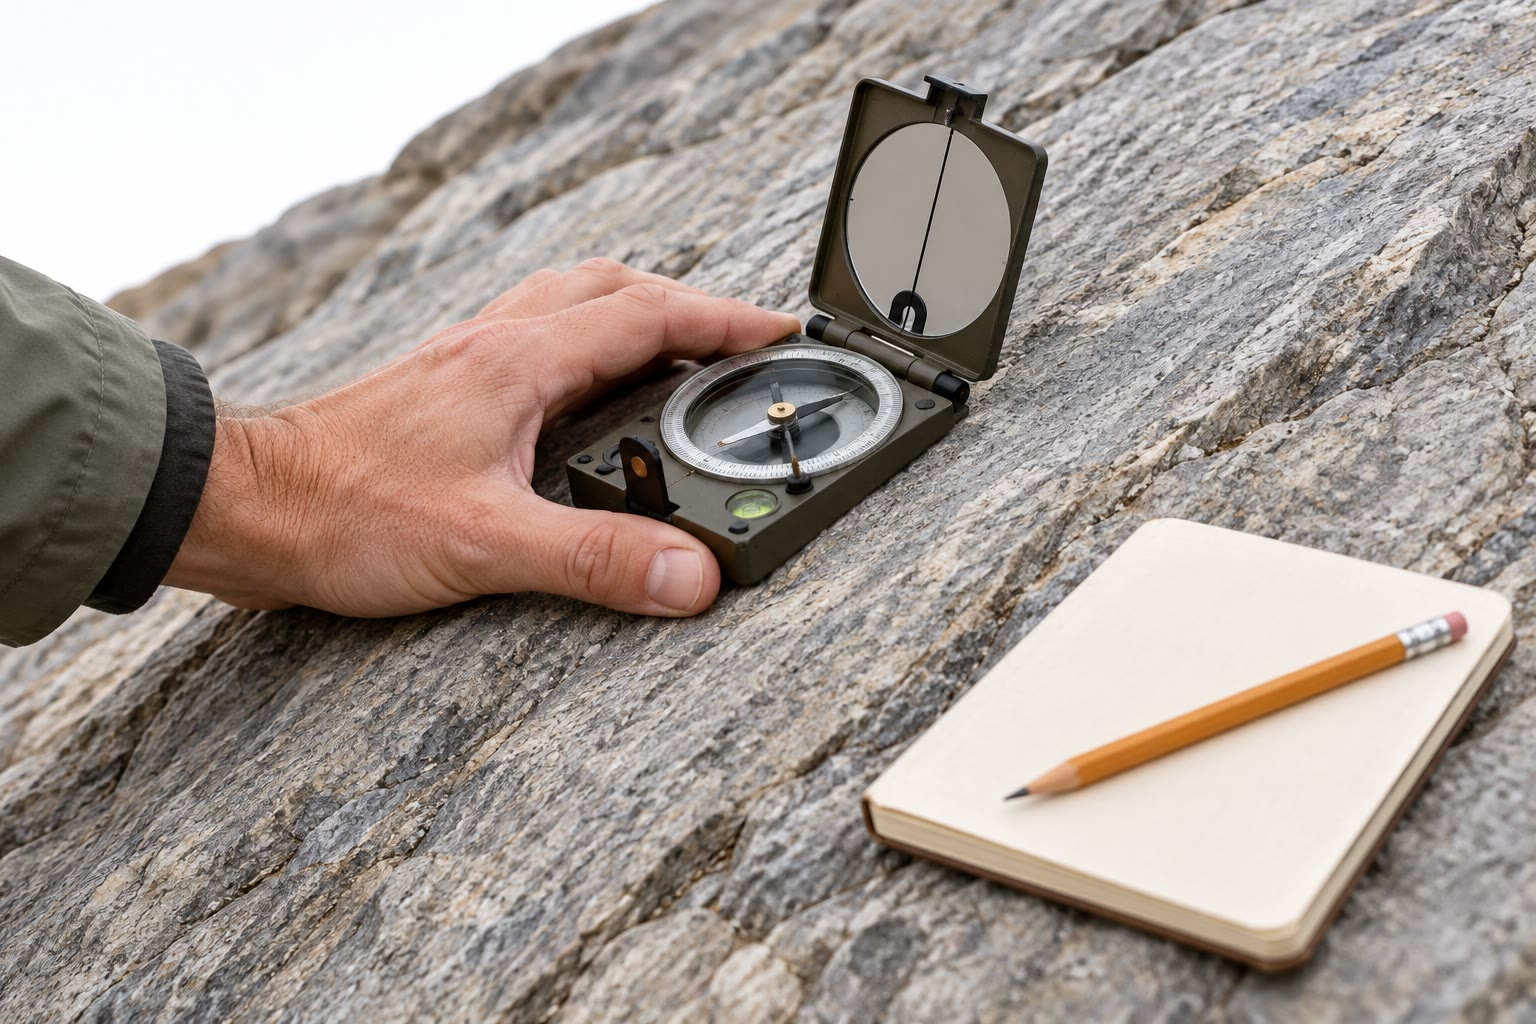
\includegraphics[width=\linewidth]{images/book5/ai/b3-compass-clinometer.jpg}

{\scriptsize Een kompas-clinometer tegen een hellend rotsoppervlak gelegd, met een
veldnotitieboekje. Door AI gegenereerde illustratie.}
\end{minipage}
\end{inthefield}

\section{Oefeningen}

\begin{exercise}[$\star$]\label{exo:b3:structural-analysis:1}
Geef de azimut en duik van de \omterm{def:b3:structural-analysis:stereo}{pool} van het vlak $040/30$ (hellingrichting,
helling). Geef de ligging van het vlak waarvan de \omterm{def:b3:structural-analysis:stereo}{pool} een azimut van \ang{315} heeft en een duik van
\ang{20}.
\end{exercise}

\begin{exercise}[$\star$]\label{exo:b3:structural-analysis:2}
Een lijn duikt onder \ang{30}. Op welke afstand van het middelpunt wordt hij getekend op een
\omterm{def:b3:structural-analysis:stereo}{hoekgetrouw net} en op een oppervlaktegetrouw net, beide met straal \qty{10}{cm}?
\end{exercise}

\begin{exercise}[$\star$]\label{exo:b3:structural-analysis:3}
De flanken van een plooi hebben de liggingen $090/30$ en $270/30$. Bereken de
hoek tussen hun polen met het inproduct van de normalen, de interflankhoek
en de klasse van de plooi.
\end{exercise}

\begin{exercise}[$\star$]\label{exo:b3:structural-analysis:4}
Een breuk $090/60$ draagt striaties met rake \ang{-45}. Met de strekkingsvector
$\vec s = (0, 1, 0)$ en de vector naar beneden langs de helling $\vec d$ van het vlak, de
glijding van de hangende wand is $\vec u = \cos r\,\vec s - \sin r\,\vec d$. Bereken
$\vec d$, $\vec u$, en de azimut en duik van de glijding. Noem de breuk.
\end{exercise}

\begin{exercise}[$\star\star$]\label{exo:b3:structural-analysis:5}
De flanken van een plooi hebben de liggingen $060/40$ en $250/30$. Bereken de
azimut en duik van de as, en de interflankhoek.
\end{exercise}

\begin{exercise}[$\star\star$]\label{exo:b3:structural-analysis:6}
Bereken de fractie van het oppervlak van het net dat binnen de cirkel ligt van
lijnen met een duik van meer dan \ang{60}, op het oppervlaktegetrouwe en het hoekgetrouwe
net, en de fractie van de richtingen op de onderhelft die
meer dan \ang{60} duiken. Welk net moet worden gebruikt om polen te tellen?
\end{exercise}

\begin{exercise}[$\star\star$]\label{exo:b3:structural-analysis:7}
Drie polen liggen in het verticale oost--west-vlak, op \ang{-20}, $0$ en
\ang{20} van de verticaal: $\vec p = (\sin a, 0, -\cos a)$. Bereken hun
\omterm{def:b3:structural-analysis:orientation-tensor}{oriëntatietensor}, de eigenwaarden en eigenvectoren, en de \omterm{def:b3:structural-analysis:pi}{bèta-as}. Waarom
is de kleinste eigenwaarde precies nul?
\end{exercise}

\begin{exercise}[$\star\star$]\label{exo:b3:structural-analysis:8}
Plaats in het Flinn-diagram het ellipsoïde $X : Y : Z = 3 : 1.5 : 1$, daarna het
ellipsoïde met constant volume met $X = 1.8$ en $Y = 1.1$. Bereken $k$ voor
elk en noem de rek.
\end{exercise}

\begin{exercise}[$\star\star$]\label{exo:b3:structural-analysis:9}
In een doorsnede evenwijdig aan de rekrichting zijn aanvankelijk ronde oöïden
nu ellipsen met een axiale verhouding $2.25$, allemaal evenwijdig, en het oppervlak van elk
is ongewijzigd. Bereken de hoofdrekken en de uitrekking langs de lange
as. Voor de rek lagen de oöïdmiddelpunten nooit dichter bij elkaar dan
\qty{0.4}{mm}: geef de halve assen van de leegte in het Fry-diagram.
\end{exercise}

\begin{exercise}[$\star\star\star$]\label{exo:b3:structural-analysis:10}
Op $\theta = \ang{60}$ vanaf het nadir, bereken de rek langs de straal,
$\mathrm dr/(R\,\mathrm d\theta)$, en langs de cirkel, $r/(R\sin\theta)$,
voor beide projecties. Controleer de stelling op de projecties, en geef de verhouding
van de assen van de ovaal waarin het oppervlaktegetrouwe net een zeer kleine
cirkel daar omzet.
\end{exercise}

\begin{exercise}[$\star\star\star$]\label{exo:b3:structural-analysis:11}
In een regime van horizontale verschuiving is $\sigma_1$ horizontaal naar \ang{000},
$\sigma_3$ horizontaal naar \ang{090} en $\sigma_2$ verticaal. Een verticale
breuk heeft een strekking van \ang{020}. Toon zonder $\vec\tau$ te berekenen aan dat de glijding
horizontaal is voor elke $\Phi$. Bereken dan $-\vec\tau$ voor $\Phi = 0.4$ met de
normaal van het vlak $\vec n = (\cos\ang{20}, -\sin\ang{20}, 0)$ en geef de
zin van de glijding.
\end{exercise}

\begin{exercise}[$\star\star\star$]\label{exo:b3:structural-analysis:12}
Een doorsnede van \qty{20}{km} lang snijdt een reeks onthechtingsplooien. Twee horizonten
op \qty{1.0}{km} afstand van elkaar steken boven hun oorspronkelijke niveaus uit met de oppervlakten
\qty{6.0}{km^2} (onder) en \qty{7.5}{km^2} (boven). Bereken de verkorting,
de diepte van het décollement onder de onderste horizon, de oorspronkelijke lengte van
de doorsnede en haar relatieve lengteverandering.
\end{exercise}

\section{Probleem: Plooien en breuken van de Varden Hills}

\begin{problem}[{Weekendprobleem --- de plooias, de spanning van een breukenset
en het herstel van een doorsnede, in een verzonnen gebied}]
\label{pb:b3:structural-analysis:1}
% values: calc/ch08.py; figdata/bachelor-3/stereonet.py (data invented from region.py)
In de Varden Hills, het verzonnen gebied van de reeks, rust een Mesozoïsche bedekking op een
basement van schist en graniet. De bedekking is geplooid tot een rechtopstaande
antiklinaal en synklinaal met rechte flanken, daarna doorgesneden door een afschuiving. Een
geoloog mat twaalf gelaagdheidsvlakken op de twee flanken van de antiklinaal
(hellingrichting/helling, in graden):

\begin{center}
\small
\begin{tabular}{l|cccccc}
\hline
oostflank & 075/13 & 084/11 & 089/13 & 079/14 & 086/12 & 072/11 \\
westflank & 283/11 & 272/13 & 281/14 & 288/10 & 276/13 & 274/12 \\
\hline
\end{tabular}
\end{center}

De sommen van de opwaarts gerichte eenheidsnormalen van de zes metingen van elke flank zijn
$\vec S_E = (1.2583, 0.2017, 5.8604)$ en $\vec S_W = (-1.2445, 0.1886,
5.8636)$ (oost, noord, omhoog). Vijf breuken dragen striaties (hellingrichting/helling,
rake van de slip van de hangende wand): $120/60/{-90}$ (de hoofdbreuk), $150/55/{-76}$,
$090/65/{-108}$, $200/70/{-78}$ en $060/50/{-105}$. De hoofdbreuk heeft een
verticale verplaatsing van \qty{200}{m}. De as van de antiklinaal en die van de synklinaal liggen \qty{4}{km} uit elkaar,
zodat de plooien zich van oost naar west elke \qty{8}{km} herhalen.

\medskip\noindent\textbf{Deel I --- Polen en de bèta-as.}
\begin{enumerate}
  \item Geef de strekking en duik van de \omterm{def:b3:structural-analysis:stereo}{pool} van de meting $075/13$, en
        zijn afstand tot het middelpunt van een oppervlaktegetrouw net met straal
        \qty{10}{cm}.
  \item Bereken de opwaarts gerichte eenheidsnormaal van de meting $075/13$; controleer die
        op grootte tegen $\vec S_E$.
  \item Bereken de gemiddelde oriëntatie van elke flank uit $\vec S_E$ en $\vec S_W$,
        de gemiddelde resultantelengten, en de kwadratisch gemiddelde spreiding van de
        metingen rond hun gemiddelden.
  \item Bereken $\vec S_E\times\vec S_W$, en de strekking en duik van de
        \omterm{def:b3:structural-analysis:pi}{bèta-as}.
  \item Bereken de hoek tussen de twee gemiddelde normalen, de interflankhoek,
        en de klasse van de plooi.
  \item Het assenvlak van deze symmetrische plooi bevat de \omterm{def:b3:structural-analysis:pi}{bèta-as} en staat
        loodrecht op $\vec m_E - \vec m_W$, het verschil van de gemiddelde
        eenheidsnormalen. Geef de oriëntatie ervan; is de plooi rechtopstaand?
  \item Geef de oriëntatie van de $\pi$-gordel, en zeg waarom de polen
        erop liggen.
\end{enumerate}

\medskip\noindent\textbf{Deel II --- De oriëntatietensor.}
De \omterm{def:b3:structural-analysis:orientation-tensor}{oriëntatietensor} van de twaalf polen is
\[
  T = \begin{pmatrix} 0.04400 & 0.00035 & 0.00109\\ 0.00035 & 0.00144 & 0.03179\\
  0.00109 & 0.03179 & 0.95456 \end{pmatrix},
\]
met de eigenwaarden $0.95562$, $0.04400$ en $0.00038$.
\begin{enumerate}[resume]
  \item Controleer dat het spoor van $T$ gelijk is aan 1. Met $\vec b = (0.0053, -0.9994,
        0.0333)$, de eenheidsvector langs $\vec S_E\times\vec S_W$, bereken
        $\vec b^{\mathsf T}T\vec b$. Wat zegt het resultaat over $\vec b$?
  \item Bereken de kwadratisch gemiddelde hoek tussen de polen en de gordel.
  \item Verklaar de waarde van $\lambda_2$ uit de hellingen van de flanken.
  \item Is de plooi cilindrisch binnen de nauwkeurigheid van de metingen?
  \item De duik van de \omterm{def:b3:structural-analysis:pi}{bèta-as} wordt bepaald door de noord--zuid-kanteling van de
        gordel, waarbij elke \omterm{def:b3:structural-analysis:stereo}{pool} bijdraagt met de spreiding die in
        vraag 9 is gevonden. Schat de standaardfout van de duik.
\end{enumerate}

\medskip\noindent\textbf{Deel III --- De paleospanning.}
\begin{enumerate}[resume]
  \item Wat voor breuk is de hoofdbreuk? Volgens Anderson, geef de
        richtingen van $\sigma_1$, $\sigma_2$ en $\sigma_3$.
  \item Toon aan, met de stelling over de sliprichting, dat de hoofdbreuk
        recht langs zijn helling omlaag glijdt voor elke waarde van $\Phi$. Wat zegt het
        over $\Phi$?
  \item Bereken voor de breuk $150/55$ de vector $\vec n$ en zijn componenten $n_1 =
        \vec n\cdot\vec e_1$ en $n_2 = \vec n\cdot\vec e_2$, met $\vec e_1$
        verticaal en $\vec e_2$ horizontaal naar \ang{030}.
  \item De slip ervan geeft $\vec w = \vec n\times\vec u = (0.771, 0.605, 0.198)$.
        Bereken $\Phi$.
  \item De andere drie kleine breuken geven $\Phi = 0.294$, $0.301$ en
        $0.306$. Geef het gemiddelde, en zeg waar de spreiding vandaan komt.
  \item Wat zegt $\Phi = 0.3$ over $\sigma_2$?
  \item Bereken de P- en T-assen van de hoofdbreuk (onder \ang{45} met het
        vlak, in zijn hellingvlak), en vergelijk ze met $\sigma_1$ en
        $\sigma_3$.
\end{enumerate}

\medskip\noindent\textbf{Deel IV --- Herstel van een oost--west-doorsnede.}
\begin{enumerate}[resume]
  \item Bereken de schijnbare helling van de oostflank, $080.9/12.3$, op een
        oost--west-doorsnede.
  \item Neem de flanken op de doorsnede onder \ang{12}, bereken de herstelde
        lengte van één plooigolflengte, de verkorting en de
        relatieve lengteverandering.
  \item Bereken de hoogte van de antiklinaalkam boven de synklinalen en het overschot
        aan oppervlakte van één golflengte, aannemend dat de synklinalen op het
        oorspronkelijke niveau bleven.
  \item Bereken de diepte van het décollement onder de geplooide laag. Kunnen de
        plooien aan de basis van de bedekking loskomen, enkele honderden meters
        diep?
  \item Bereken de horizontale verplaatsing en de slip van de hoofdbreuk op een
        doorsnede langs \ang{120}.
  \item Bereken op de oost--west-doorsnede de schijnbare helling van de breuk en
        haar schijnbare horizontale verplaatsing. Welke doorsnede moet worden hersteld?
  \item In welke volgorde worden de breuk en de plooien hersteld, en waar worden de
        \omterm{def:b3:structural-analysis:restoration}{pinlijnen} geplaatst?
  \item Wat is de duik van de plooias van de Varden, afgeleid uit de twaalf
        metingen?
\end{enumerate}
\end{problem}
